% This chapter should describe what was actually produced: the programs which were written, the hardware which was
% built or the theory which was developed. Any design strategies that looked ahead to the testing stage might 
% profitably be referred to (the professional approach again).

% Descriptions of programs may include fragments of high-level code but large chunks of code are usually best left % to appendices or omitted altogether. Analogous advice applies to circuit diagrams.
% Draw attention to the parts of the work which are not your own. Making effective use of powerful tools and 
% pre-existing code is often laudable, and will count to your credit if properly reported.
% It should not be necessary to give a day-by-day account of the progress of the work but major milestones may 
% sometimes be highlighted with advantage.

% ~4500 words

\documentclass[final,dissertation.tex]{subfiles}
\begin{document}

\chapter{Implementation}

In this chapter, I will describe how I implemented my project, describing challenges faced along the way. The implementation consists of the following:

\begin{itemize}
    \item \textbf{Recording signs: }This includes the code which uses OpenCV to capture frames. They also integrate most of the functionality for determining when to process a given sequence of frames, when to reset the recording, and displaying visual and textual output to the user.
    \item \textbf{Pre-processing datasets: }They help process the datasets into a suitable format for the program to read them. LSA64 has one script which does the entire processing step, whereas BSLDict has an additional script to filter labels that have less than a desired amount of data.
    \item \textbf{Extracting features from the datasets: }They are used to get the relevant features that will be used to train our model. We use mediapipe holistic to first extract landmarks from video frames, then we convert these to angles and relative distances. This is discussed further in the relevant following section.
    \item \textbf{Comparing signs: }They focus on the computation using the DTW algorithm. They include the code which return the distances between any two compared signs and also the functionality to determine if any given sign is output with a certain confidence.
\end{itemize}

\section{Data Pre-processing}

The model needs the data to be in a a required format in order to process it. As such, we need to pre-process existing datasets in order to make them suitable.

We order the videos by having a directory for each label, containing all videos which fall under that corresponding label.

\subsection*{BSLDict}

BSLDict is a large dataset of isolated BSL gestures \cite{momeni2020watch}. The data has been obtained from BSL sign aggregation platform \textit{signbsl.com}, with a total of 14k video clips for a vocabulary of 9k labels.

The data provides two main issues:

\begin{itemize}
    \item \textbf{Lack of examples per label: }A lot of the labels have only one or two videos. This is a problem as there is not enough data for testing or to use deep learning for efficient training.
    \item \textbf{Different signs per label: }Many labels contain ambiguous sign gestures. Some of the labels have different ways to represent them and some overlap with other labels as well. This leads to poor accuracy when trying to train on them.
\end{itemize}

The issue of lacking examples was one reason why DTW was used as an algorithm for this project. As deep learning models require a sufficient amount of training data to be sufficiently accurate, we use a model based on DTW instead as it can retain accuracy with less data.

\begin{figure}
    \begin{center}
        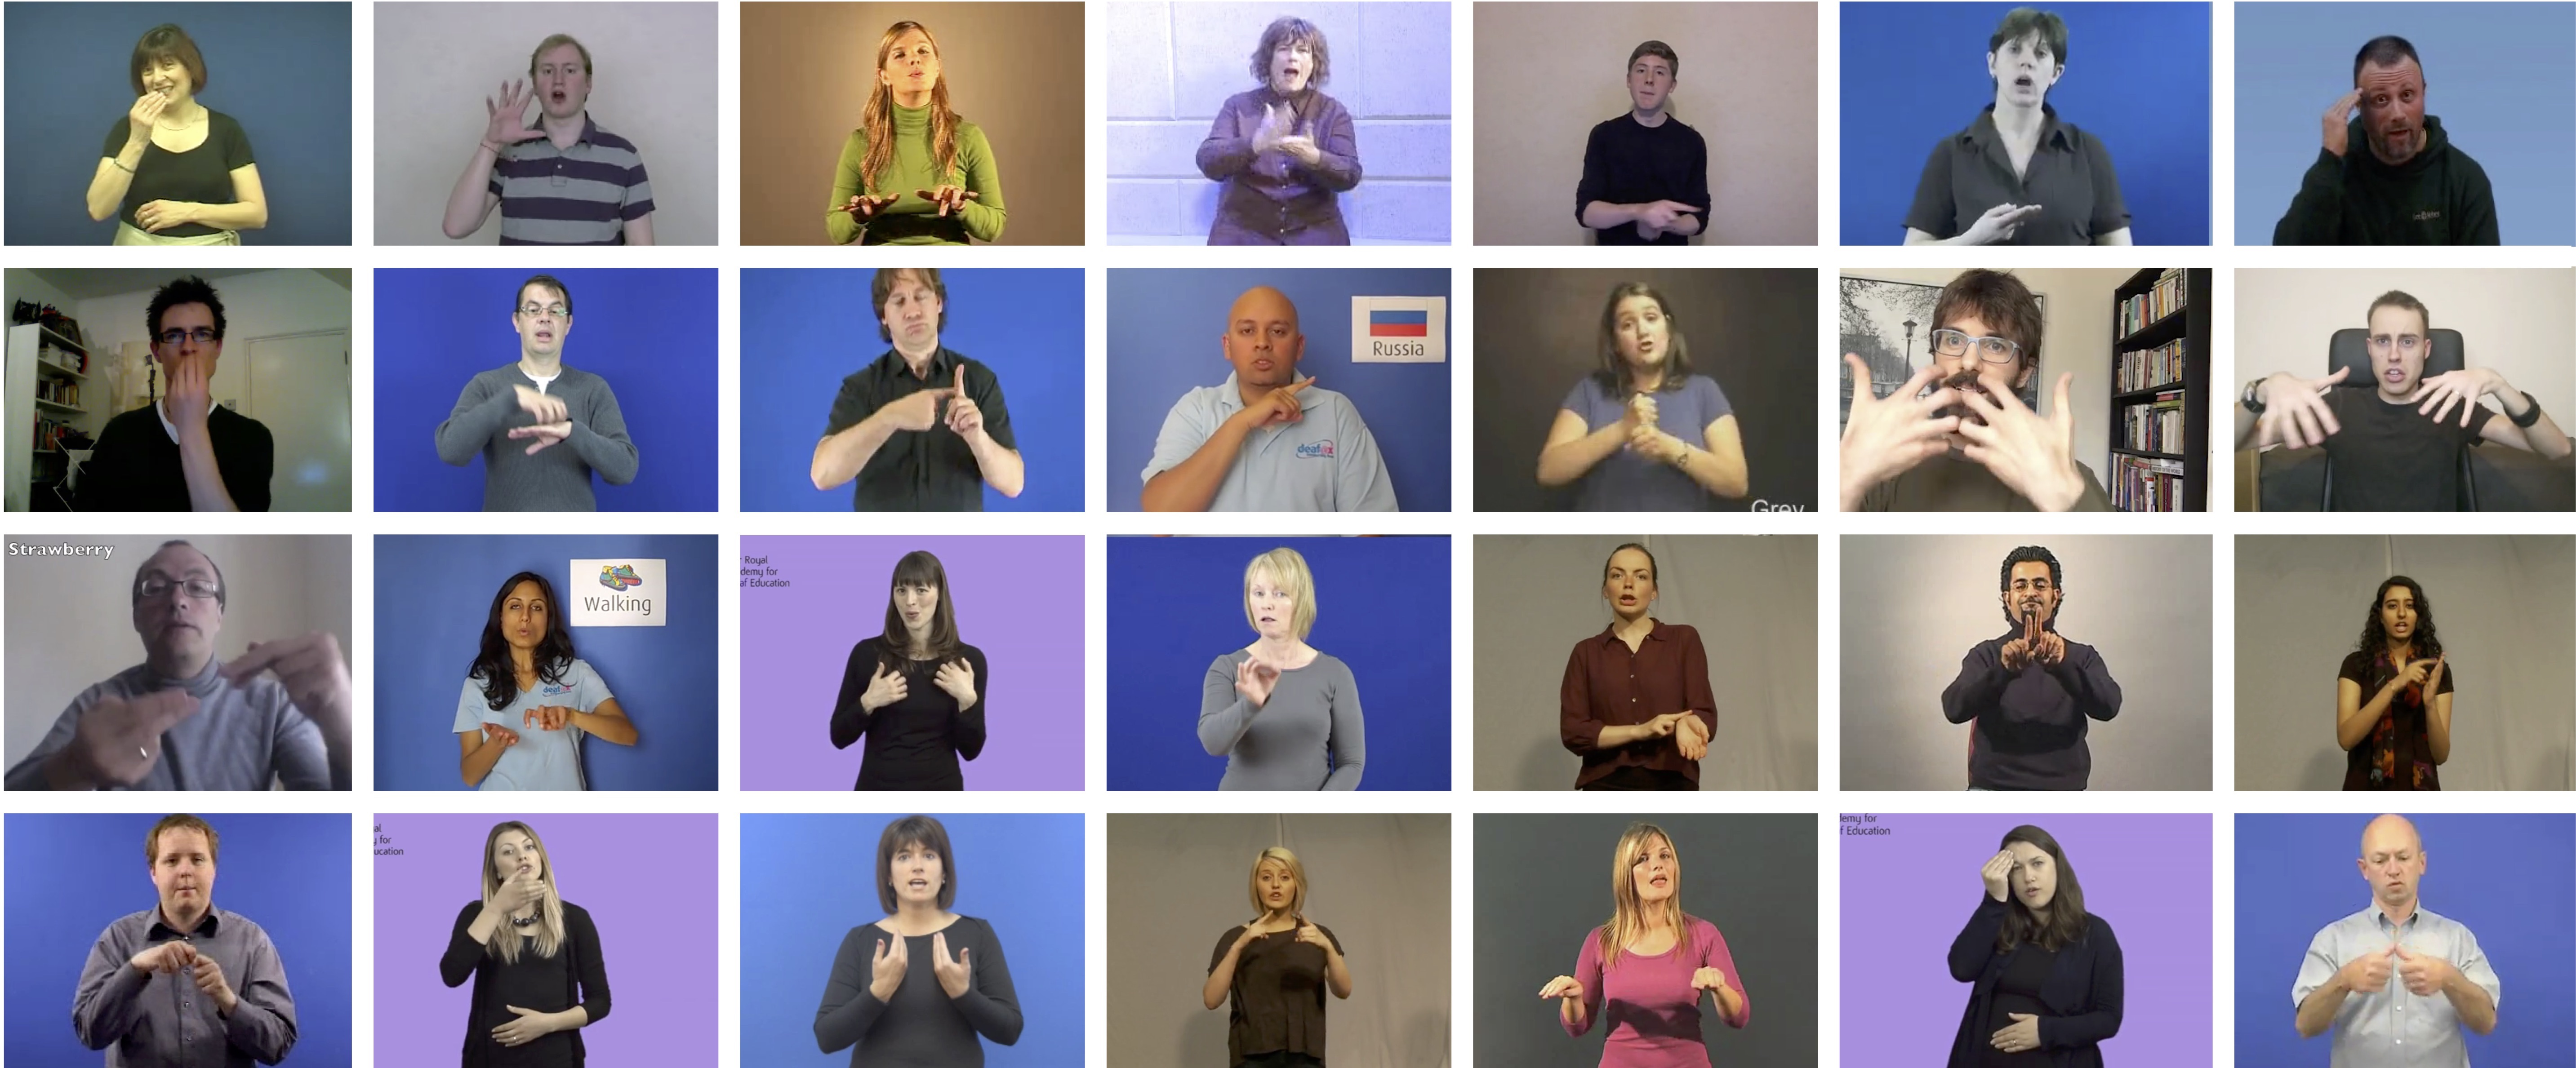
\includegraphics[scale=0.07]{images/BSLDict.jpeg}
        \caption[caption]{Examples from the BSLDict dataset}
    \end{center}
\end{figure}

\subsection*{LSA64}

LSA64 is a sign database for isolated Argentian Sign Language (LSA) gestures \cite{ronchetti2016lsa64}. It was created to produce a dictionary for LSA and to be used for training automatic sign recognition models. The dataset contains 3200 videos, with 10 signers executing 5 repetitions of 64 different types of signs.

This dataset was used mostly for initial testing purposes given the issues that were encountered with BSLDict. It provides both sufficient data and consistent signs per label.

Signers wore coloured gloves to aid hand recognition and segmentation, as well as wearing dark clothing. This does not affect this project due to the use of mediapipe to recognise signs.


\begin{figure}
    \begin{center}
        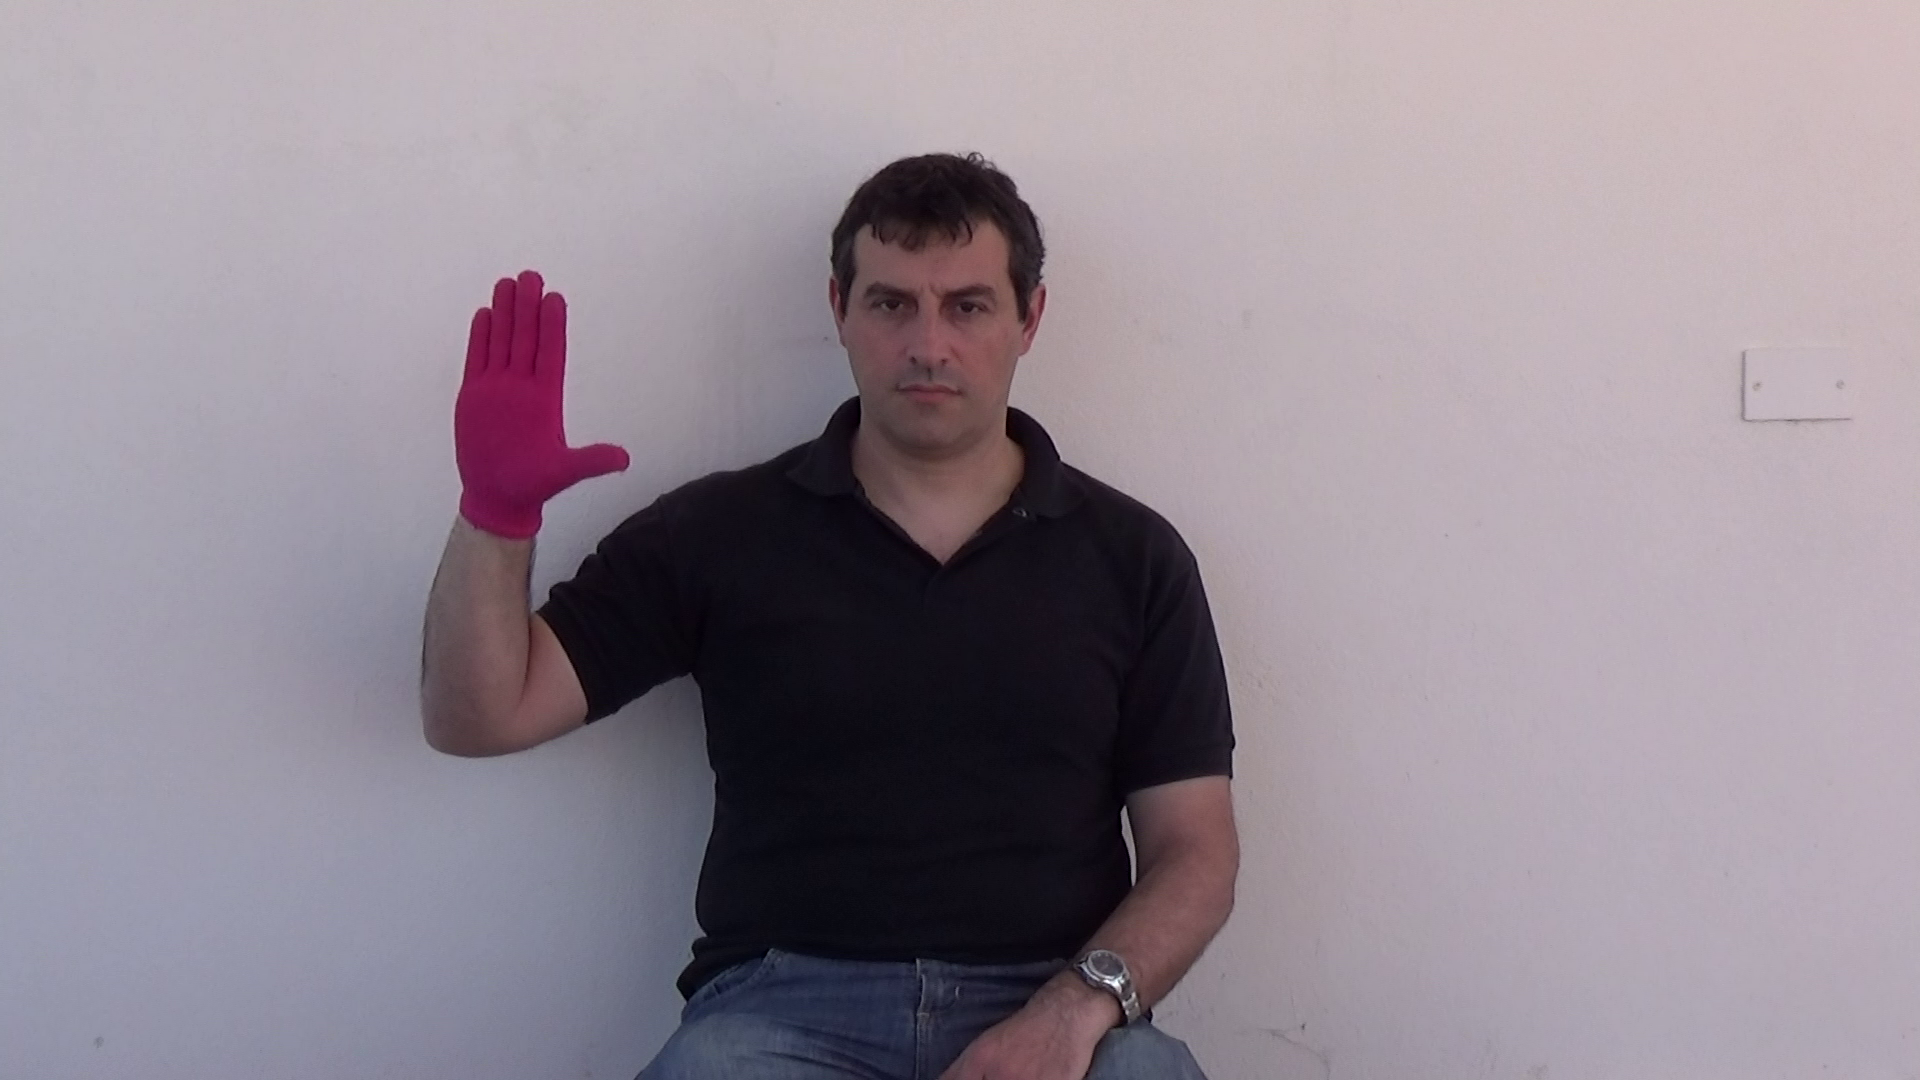
\includegraphics[scale=0.15]{images/LSA64.png}
        \caption[caption]{Snapshot from the LSA64 dataset}
    \end{center}
\end{figure}

\section{Mediapipe Extraction}

Using our datasets, we now need to extract information from them. This is done by processing each frame in a given video individually.

\subsection{Mediapipe Holistic}

Mediapipe Holistic is the model that outputs the needed data to start the feature extraction process.

Mediapipe Holistic utilizes a deep neural network model that is trained on a large dataset of labeled images and videos. The model is designed to recognize various human poses, hand gestures, and facial landmarks, and it achieves this by analyzing the pixels of the input image or video stream \cite{grishchenko_bazarevsky_2020}. Mediapipe Holistic provides three tracking pipelines, namely for the face, hands, and pose. The latter two are of relevance to this project.

\subsection{Hands Detection Pipeline}

Detecting hands with articulated fingers is a complex task, due to factors such as varying hand spans relative to image frames. Unlike faces, hands lack high-contrast areas, increasing the complexity of detecting them. As such, usage of other features such as arms and the torso can help localise hand positions more accurately.

Mediapipe employs palm detection, as boundary-estimation is relatively easier compared to hands with articulated fingers. A Single-Shot Detector model called BlazePalm is used to detect initial hand locations. An encoder-decoder feature extractor is used for bigger scene context awareness, an approach similar to RetinaNet. Further explanation about these methods are described below.

\subsubsection{Single-Shot Detection}

Single Shot MultiBox Detector (SSD) is a state-of-the-art object detection algorithm that was proposed by Liu et al. in 2016 \cite{liu2016ssd}. SSD is a single-shot detector, which means that it can detect objects in a single forward pass through the network. This makes SSD much faster than two-stage detectors like R-CNN and Fast R-CNN, which require two forward passes through the network.

SSD works by predicting a set of bounding boxes and confidence scores for each object in an image. The bounding boxes are predicted using a set of anchor boxes, which are predefined boxes that are placed at different locations and scales in the image. The confidence scores are predicted for each anchor box, indicating how likely it is that the anchor box contains an object.

After the bounding boxes and confidence scores have been predicted, they are used to generate a set of final detections. This is done by first applying non-maximum suppression (NMS) to the bounding boxes. NMS is a technique that is used to remove duplicate detections. In NMS, the bounding boxes are sorted by their confidence scores, and then the boxes that have a high overlap with other boxes are removed.

After NMS has been applied, the remaining boxes are then classified using a softmax classifier. The softmax classifier outputs a probability distribution over the set of object classes. The class with the highest probability is then assigned to the box.

SSD has been shown to be very effective for object detection. It has achieved state-of-the-art results on a number of benchmark datasets, including the PASCAL VOC dataset and the COCO dataset. SSD is also very fast, making it suitable for real-time object detection applications.

\subsubsection{Non-Maximum Suppresion}

Non-maximum suppression (NMS) is a technique used in computer vision to eliminate duplicate or redundant detections of the same object in an image. It is commonly used in object detection tasks such as pedestrian detection, face detection, and vehicle detection. The algorithm works by selecting the detection with the highest confidence score and suppressing any overlapping detections that have a lower confidence score.

The NMS algorithm can be described mathematically as follows:

Given a set of bounding boxes, $B = {b_1, b_2, ..., b_n}$, and their corresponding confidence scores, $S = {s_1, s_2, ..., s_n}$, where $n$ is the number of bounding boxes, the goal is to select a subset of bounding boxes, $B^* \subseteq B$, that have a high confidence score and do not overlap significantly with each other.

First, we sort the bounding boxes in descending order of their confidence scores. Let $b_i$ be the bounding box with the highest confidence score, i.e., $s_i = \max_{j=1}^{n} s_j$. We add $b_i$ to the subset $B^*$ and remove it from the set $B$.

Next, we calculate the Intersection over Union (IoU) between $b_i$ and each of the remaining bounding boxes $b_j \in B$, where $j \neq i$. The IoU is defined as:

\begin{equation*}
    \text{IoU}(b_i, b_j) = \frac{\text{area}(b_i \cap b_j)}{\text{area}(b_i \cup b_j)}
\end{equation*}

If $\text{IoU}(b_i, b_j) > \text{threshold}$, where $\text{threshold}$ is a predetermined threshold value (e.g., 0.5), we remove $b_j$ from the set $B$. We repeat this process until all the bounding boxes in $B$ have been processed.

The final output is the set $B^*$ of selected bounding boxes.

The NMS algorithm helps to reduce the number of false positives and improves the accuracy of object detection models by removing redundant detections.

\subsection{Pose Detection Pipeline}

The process for pose detection, BlazePose, is similar to that used for hands \cite{bazarevsky2020blazepose}. The BlazePose detection pipeline consists of a lightweight pose detector followed by a pose estimation component.

\subsubsection{Pose Detection}

The first stage of the BlazePose pipeline is body part detection. Unlike the hands detection pipeline, BlazePose does not use the NMS algorithm as it breaks down in cases where poses are highly articulated. This is because multiple bounding boxes satisfy the IoU threshold. Instead, a face detector is used as a proxy for the person detector. This is augmented with additional person alignment parameters such as the middle point between the person's hip. The CNN used in the face detector is based on the BlazeFace architecture \cite{bazarevsky2019blazeface}, which uses a modified MobileNetV1 model with depth-wise separable convolutions.

\subsubsection{Pose Estimation}

The pose estimation component predicts the location of the 33 landmarks, using the bounding boxes that were obtained from the first stage.

To achieve accurate pose estimation, a combined heatmap, offset, and regression approach is adopted. During training, the heatmap and offset loss are used to supervise the model, but the corresponding output layers are removed before running inference. This approach effectively uses the heatmap to supervise a lightweight embedding, which is then used by the regression encoder network. This approach is inspired by the Stacked Hourglass approach of Newell et al. \cite{newell2016stacked}, but in this case, a tiny encoder-decoder heatmap-based network is stacked with a subsequent regression encoder network.

To achieve a balance between high- and low-level features, skip-connections are actively utilized between all the stages of the network. However, the gradients from the regression encoder are not propagated back to the heatmap-trained features. This approach not only improves the heatmap predictions but also substantially increases the coordinate regression accuracy.

\subsection{Mediapipe Pipeline}

One problem with using multiple separate models is that each is optimised for their specific purposes \cite{grishchenko_bazarevsky_2020}. For example, the pose estimation model requires a $256 \times 256$ input video frame. However, cropping the hand and face from this frame to feed their respective models results in an input which has a too low resolution to obtain accurate landmarks.

To solve this, Mediapipe Holistic uses a multistage pipeline. First, the human pose is estimated using the pose pipeline. Using the inferred pose landmarks, it then derives the regions of interest (ROI) for the face and hands, employing a recrop model along the way to improve it. The ROIs are then passed into the respective models to obtain the remaining landmarks.

\begin{figure}[H]
    \begin{center}
        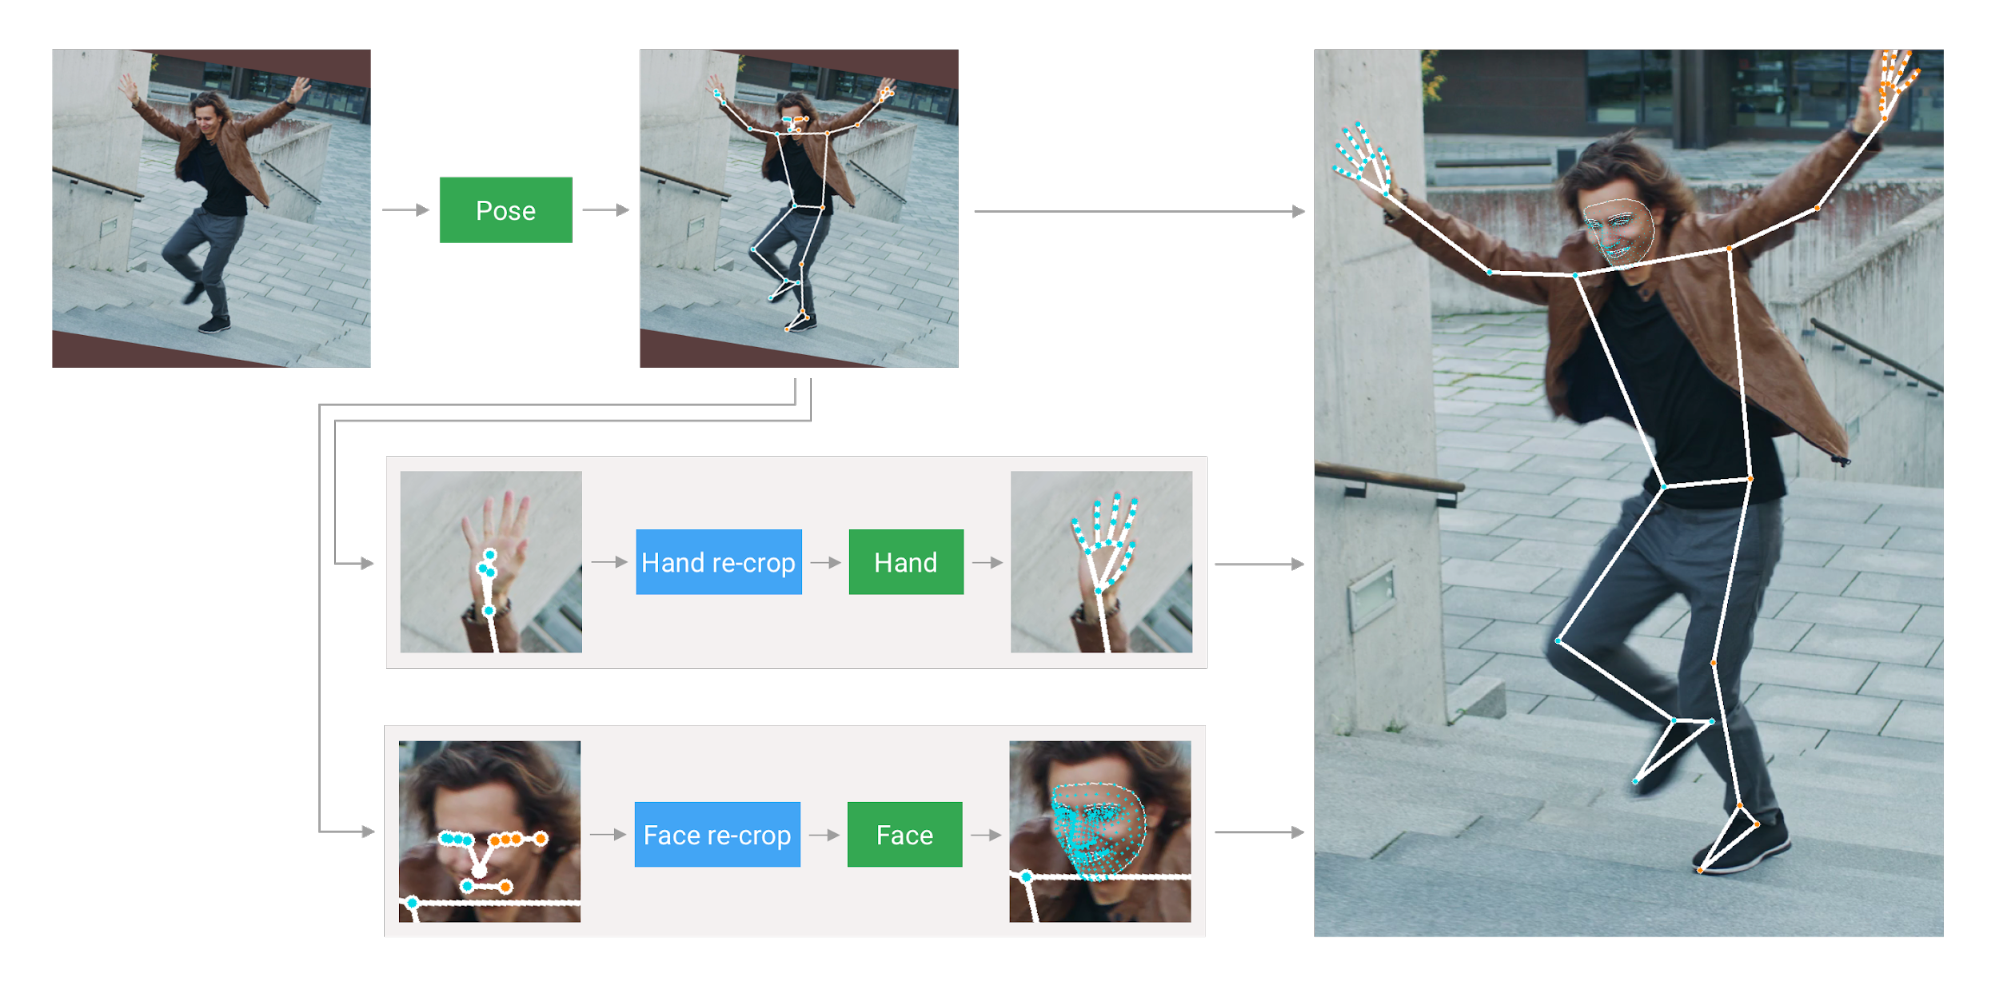
\includegraphics[width=\textwidth]{images/holistic_pipeline.png}
        \caption[caption]{Pipeline Overview}
    \end{center}
\end{figure}

\subsection{Mediapipe Implementation}

The goal here is to obtain the position of the different connections between joints.
\newline \verb|mediapipe_utils| provides methods which help in locating the landmarks given a frame. The detection is relatively straightfoward to implement, using the provided Holistic model that is imported as part of the library. We can just use the model's \verb|process| method. We also have to do color conversion because frames from OpenCV use BGR color rather than RGB. To add visual representation to the frames, the method \verb|draw_landmarks| can be used to add drawing specifications to display the landmarks and the connections between them.

\begin{figure}[H]
    \begin{center}
        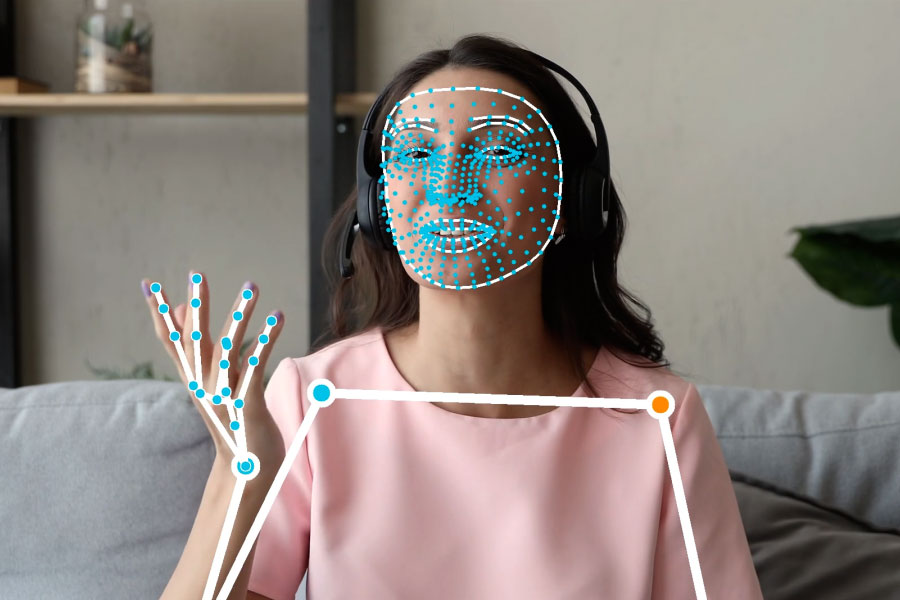
\includegraphics[scale=0.3]{images/holistic.jpg}
        \caption[caption]{Visual display of landmarks of Mediapipe Holistic (Image from mediapipe.dev)}
    \end{center}
\end{figure}



\section{Feature Extraction}

Once a list of connections from mediapipe has been obtained, we want to store this data in a suitable format and being able to reload them. The \verb|feature_extraction| script provides a range of methods to do so. The initial training stage involves obtaining a collection of reference signs. These are what the recorded signs will be compared to to evaluate similarity.

\subsection{Extract to Pickle Files}

Initially, the \verb|extract_features| method is used to obtain the landmarks from the data in our training folder. Every video is scanned and the relevant data extracted by mediapipe is stored in pickle files.

We use this opportunity here to also extract the data of the laterally-inverse of the frames. The reason for this is to obtain the features of the sign performed in a left-handed manner. In BSL, the leading hand used to perform the signing determines the handedness of the sign. Thus, flipping the image is sufficient to obtain the relevant data.

Each training video has two entries corresponding to it: its own extracted data and its flipped data. Each entry contains a pickle file for each hand and the pose, which is essentially an array of landmarks.

\subsection{Loading Reference Signs}

To perform predictions, the reference data needs to be loaded for the session. The \verb|load_reference_signs| method is used to iterate through the entries containing the pickle files. For each entry, we initialise a new \verb|sign_model| object, which is itself initialised with the respective \verb|hand_model| and \verb|pose_model| objects constructed from the data stored in the pickle files.

For efficiency, we use a \verb|pandas.DataFrame| to store the name of the sign, its respective \verb|sign_model|, and a distance initialised to 0. This will be overwritten when computing the distances.

\section{Models}

The project uses three models to represent features extracted from the vectors provided by Mediapipe Holistic.

\subsection*{Hand Model}

The \verb|hand_model| stores the feature vector representing all the angles between the connections provided by mediapipe on an arbitrary hand. Mediapipe provides 21 connections per hand, resulting in a feature vector of $21 * 21 = 441$ angles. We use the dot product formula to obtain the angle given two vectors (See Figure 3.2):

\begin{equation*}
    \theta = cos^{-1}\Big(\frac{a \cdot b}{|a| |b|}\Big) \text{, where $a$ and $b$ represent connections}
\end{equation*}

The model only represents one particular frame, given a sequence of them. The final sign gesture is thus represented by a sequence of hand models.

\begin{figure}[H]
    \begin{center}
        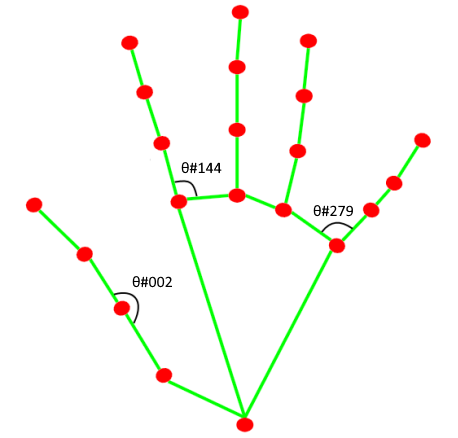
\includegraphics[scale=0.7]{images/hand_landmarks.png}
        \caption{The angles on the mediapipe connection drawing}
    \end{center}
\end{figure}


\subsection*{Pose Model}

The \verb|pose_model| takes a different approach. Instead of using angles, we use the distance between the shoulder and elbow as a normalisation distance, normalising coordinates provided by mediapipe. This is because the pose landmarks also include those of the lower body, including the legs. Hence, we only use the landmarks of the shoulder, elbows and wrist, as they are more likely to be present in the frames. Taking $a$ and $b$ as the position vectors representing the shoulder and elbow respectively, we obtain the new coordinates as follows:
\begin{equation*}
    v_i = \frac{u_i}{|b - a|} \text{, for every coordinate $u$ in the pose landmarks}
\end{equation*}

\begin{figure}
    \begin{center}
        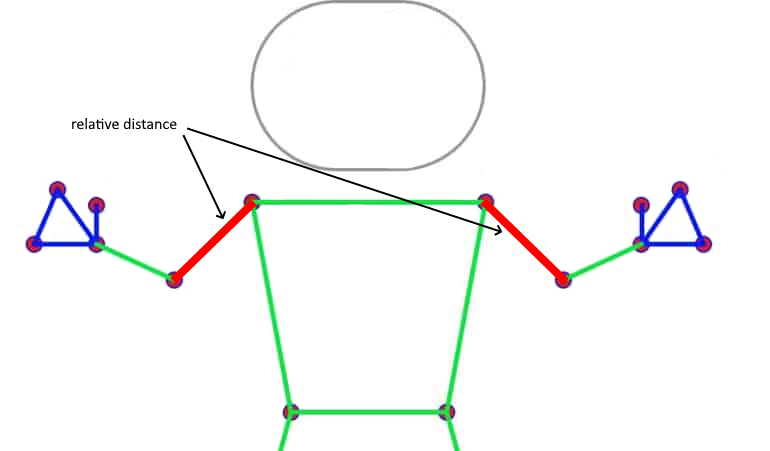
\includegraphics[width=\textwidth]{images/pose.png}
        \caption{The relative distance used to normalise the landmarks}
    \end{center}
\end{figure}

\subsection*{Sign Model}

The \verb|sign_model| object stores the hand and pose models for each frame in the sequence representing the sign, essentially being the representation of the sign as its features. This is what is compared when computing the similarity between a reference sign and a recorded sign.

Each object contains the following attributes:

\begin{itemize}
    \item \verb|has_left_hand| and \verb|has_right_hand|, which are booleans which are true if such hand is present in the video.
    \item \verb|lh_embedding| and \verb|rh_embedding|, which are the lists of feature vectors for each frame for each hand.
    \item \verb|left_arm_embedding| and \verb|right_arm_embedding|, which are the lists of feature vectors for each frame for each arm.
\end{itemize}

\section{Computing Similarity}

The project provides two scripts for computing similarity: \verb|compute_dtw| and\newline \verb|compute_fastdtw|, which use the \verb|dtw-python| and \verb|fastdtw| libraries respectively. The project provides an easy way to toggle between the two algorithms.

\subsection{dtw-python}

The \verb|dtw_distances| method is what fills the \verb|pandas.DataFrame| with distances. It takes the DataFrame as an argument along with the sign model representing the recorded sign. The embeddings of the sign model are extracted to variables as they are the sequences to be compared.

The model starts iterating through every sign present in the DataFrame. It discards those which do not have the same hands present in the recorded sign and sets their distances as $\inf$ in the distance column of the DataFrame. The \verb|dtw| method from \verb|dtw-python| \cite{giorgino2009computing} is then called with the respective embeddings of the reference and recorded sign as arguments. The distance obtained is then set in the corresponding entry of the DataFrame.


\subsubsection{Challenges Faced}

The \verb|dtw| method handles the case of having a sequence of length 1 differently. In such a case, it transposes the array. This happened in a few instances on training due to some signs registering a particular hand in only one frame. This is dependent on the confidence tracking of mediapipe. As such, this specific case is handled by duplicating the singular entry present in the sequence to obtain an array of length 2.

\subsection{fastdtw}

The \verb|fastdtw_distances| method works similarly to \verb|dtw_distances|. It uses the \verb|fastdtw| instead to calculate the distances. This implementation does not suffer from the same issue of handling sequences of length 1. This implementation runs in linear time, rather than in O$(m \times n)$.

\section{Sign Prediction}

Given the \verb|pandas.DataFrame| with all distances computed, a prediction can now be made. The DataFrame is first sorted in ascending order of distances, with the top row being the sign with the lowest distance. Lower distances indicate higher similarity.

\subsection{Batch Size and Threshold}

The \verb|get_sign_predicted| method takes an argument for \verb|batch_size|. This indicates how many signs we need to consider in order to make a reliable prediction. For example, we can take a batch size of 5, which means we take the 5 signs with the lowest distances and output the most common one. This increases the confidence in the prediction made. We choose a label $l$ as follows:

\begin{equation*}
    l = \max\Big(\frac{l_i}{N}\Big) \text{, for $0 \leq i < N$}
\end{equation*}

$N$ corresponds to the chosen \verb|batch_size|. A reasonable upper bound for $N$ can be obtained by considering the label in the training data with the least amount of examples. This ensures that every label has the possibility of achieving a confidence of 100\%.

The threshold argument is used to determine if a sign is common enough to be output with a certain minimum confidence. It is defined as the minimum ratio of appearances to the batch size that a sign needs to achieve in order to be output.
The model outputs ``Unknown Sign'' if the threshold is not met.

\section{Usage}

The implementation provides a record button to start a capture of a determined number of frames. Once pressed, the feed will capture that amount of frames and process them. To indicate that the feed is recording, a circle is used as an indicator. It turns red while the feed is recording.

A hand and pose model will be generated for each frame and they are all stored in a sign model. Once compared, the program will output the most probable label as a prediction, which will be displayed on the bottom of the feed.




\end{document}